\chapter{Literature review}
\label{mathchapter}
\section{Background}
In this chapter, a review of active queue management schemes to address the congestion control in WSN is presented. Firstly,it discusses various congestion control approaches in the existing literature followed by active queue management schemes. Finally, the chapter is concluded with the research gap in the existing literature motivating the objectives for the work undertaken.
\section{Key related research}
\subsection{Related work on congestion control}
In WSN, large number of nodes are deployed in the sensor fields to report any event. The 
A. Ghaffari[9] provided a well-organized work unfolding the exact functionality and techniques employed within the existing literature and comparative study is performed. The papers that were reviewed in the survey were balanced in numbers and presented the latest congestion control schemes that enabled us to get effectively benefited from the complete literature review. It provides a comprehensive survey having the detailed review of old as well as the latest congestion control schemes, provides the taxonomy, and identifies open research issues.
\par 
In Nikokheslat[15], a congestion control algorithm is proposed in which an alternative route is
produced between the source and the sink nodes to prevent the presented and evaluated congestion. The proposed method is dynamic in nature since it make use of  local information such as the degree of congestion on nodes' neighbor to change the path of routing in order to prevent the occurrence of congestion. The proposed algorithm uses the following four steps to make an alternative route:
\begin{itemize}
    \item Controlling topology
    \item Producing a hierarchical tree
    \item Producing an alternative route
    \item Managing nodes with energy shortage
\end{itemize}
\par 
In paper[15] initially, local minimum spanning tree was used to control topology in the network. The property of local minimum spanning tree is that it can establish communication in a way that each node has a certain number of neighbor nodes. 
\par 
In WSN, there are data with different priorities; their transmission should be done fairly and justly. The paper considers three different types of data: real-time, fast and normal traffic. Real-time traffic has been given half of the priority, as they are delay-sensitive.  Remaining of 30\% priority is given to the fast traffic and the rest 20\% was assigned to normal traffic. The second strategy implemented in this paper is that if any of the buffers do not have the intended value or if the amount of data to be transmitted is less, the other buffers will be given priority. That is, first priority will be given to the real time traffic, else fast traffic will be assigned the same. In situations where there is no fast traffic,  allocation will be done to normal traffic.
\par 
The proposed mechanism relies heavily on controlling the topology of the network. The parameters considered are throughput, packet delivery ratio and network lifetime. Further, these parameters are calculated assuming that six neighbour nodes are sufficient to generate the topology. End-to-end delay, another important parameter for WSNs' has not been discussed. 
\par
In Ahmed[1] congestion avoidance and mitigation (CAM) protocol is used to avoid and control congestion by data-rate adjustment.Figure 2.1 shows the work flow of this protocol which is explained below.
\begin{figure}[H]
    \centering
    \includegraphics[scale=0.7]{Thesis/figs/8.png}
    \caption{Work Flow of Congestion avoidance and mitigation protocol}
    \label{fig:my_label}
\end{figure}
The distance between each pair of sender and receiver is used to select the route. RSR is the relative success rate given by :
{\begin{center}
     Relative success rate = $\frac{NoPTx}{NoPFx}$
\end{center}}
where NoPTx and NoPFx are the number of packets transmitted at the MAC layer and number of packets forwarded at the network layer, respectively, for a given period of interval.
%\begin{figure}[H]
    %\centering
    %\includegraphics[scale=0.7]{8.png}
    %\caption{Work Flow}
    %\label{fig:my_label}
%\end{figure}
\par
To do that, routes are selected by three parameters, i.e., the distance between sender and receiver, RSR value of the node and buffer occupancy of a node. A utility function is calculated, and each neighbor node of a transmitter node applies the same. Hence, the highest U-valued neighbor node in the set of all neighbor node is selected as the next hop node for transmitting node in packet forwarding. Congestion is prevented by choosing non-congested nodes as its next hop node. 
\par
The utility function consists of three variables: 
\begin{itemize}
\item Distance to the next node. 
\item Relative success rate (RSR) of each neighbor node. 
\item Buffer occupancy of a node at a time to provide feedback based congestion control
\end{itemize}
The formula used to calculate the utility function is given as :
{\begin{center}
     Utility function $U(t)=p\times \frac{Lt}{L}+q \times RSRt+r \times bi(T)$
\end{center}}
Lt=distance of next node t towards the BS from node B\\
L= maximum distance covered by the transmission power of each node\\ 
RSRt = relative success rate of node t\\
bi(T) = buffer occupancy of the node at time T\\
Ullah[21] proposed a scheme for ZigBee-based WSN. It prioritizes the packets to reduce the drop rate of high priority packets.
It also tries to avoid congestion by employing multipath routing which in turn increases the delivery ratio of the packets as shown in Figure 2.2 .
\begin{figure}[h!]
    \centering
    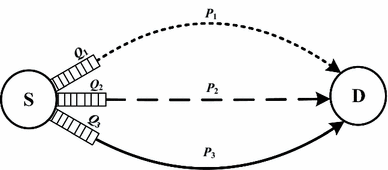
\includegraphics[scale=0.7]{Thesis/figs/2.png}
    \caption{Multipath structure}
    \label{fig:my_label}
\end{figure}
In the proposed scheme three queues, Q1, Q2, and Q3, of different queuing discipline are used for accommodating the packets of each of three priorities, respectively. Each of them is associated with a path such as Q1 with P1, Q2 with P2, and Q3 with P3. Here statistical path scheduling is applied such that if Q1 is empty, the packets in Q2 are distributed to P1 and P2. Similarly, if both Q1 and Q2 are empty, the packets in Q3 are distributed to all the three paths. With the proposed approach, different types of packets are forwarded to the receiver simultaneously on multiple paths, maximizing the path utilization. 
\subsection{Related work on active queue management}
Traditional Queue Management such as Tail Drop, is based on the FIFO policy, i.e. the packets are received at incoming links and sent out at the outgoing links. The incoming packets are enqueued in the buffer till its empty, after which the packets are simply dropped. In this mechanism, there is no prior notification to congestion detection in the network, the congested network drops the incoming packet. This causes serious shortcomings because the dropped packets are re-transmitted and it causes over-utilization of many resources such as battery and processing power of the nodes. These shortcomings do not recommend it for interactive applications in the network where the occupied buffer size remains closer to full for a larger potion of transmission time and packets are dropped once after the queue reaches its maximum length.[18] Following this, another strategy, random drop strategy was used to randomly drop any packets incoming to the queue in order to avoid the buffer getting full. 
\par
The main idea behind Active Queue Management(AQM) schemes is to monitor the buffer queue length and decide whether to discard or enqueue a packet before the buffer overflow occurs. Subsequently, the intermediate nodes predicts the congestion and notifies the source to avoid the congestion in the network. Therefore, AQM helps in improving upon the packet loss as well as reduces the queuing delay experienced by the packets in the queue. The primary goal for any AQM scheme is to maintain a steady state for the queue, preferably small in size, so that the shortcomings of Tail Drop and other similar techniques are resolved. The idea behind keeping the queue size smaller is to lower the end-to-end delay in the network.
\par
The paper[20] proposes an AQM scheme based on a priority queue, Improve RED(IRED). The probability to mark a packet and drop it, is based on the packet arrival rate and size of the queue in order to reduce the network congestion. On comparison with the traditional AQM practices(RED) indicates that their proposed algorithm not only improves on the packet loss rate but also provides a considerable steady queue size. This can be a desirable feature for any AQM scheme since 
Stability of the queue could be a desirable feature of an AQM policy since it helps in lowering the packet loss rate, and therefore the
projected policy has this distinct feature.
\par
This paper [10], concisely surveys comparative analysis
of various congestion control algorithms. The AQM
algorithms are classified based on congestion metrics and
the flow data. Most of the AQMs solely need congestion
indicators whereas a number of them need each congestion
indicator and flow data. Very few need only flow data for
detecting congestion. These AQMs are compared based on
the assorted performance metrics. This paper tries to
project the desirable quality and disadvantage that exists in
every of the algorithm in terms of their performance.
\par 
In[2][10]authors studied numerous congestion management techniques and explore
the chances of additional analysis within the space of congestion management.The Tail Drop(Drop Tail) simply drops the packets after the buffer gets full(Figure 2.3). According to them Major
downside of RED is its parameter sensitivity though by the comparison it's shown that RED performs slightly higher than Drop Tail. 
\begin{figure}[h!]
    \centering
    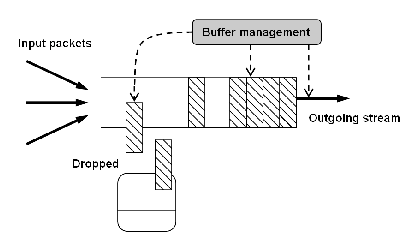
\includegraphics[scale=1.5]{Thesis/figs/fig1.png}
    \caption{Drop tail Mechanism}
    \label{fig:my_label}
\end{figure}
They concludes that until node eight RED and Drop tail performed virtually equally. From node eight until node thirty two RED performed higher than drop tail. Where as in Tail Drop, once the queue becomes full, it starts dropping packets; RED reduces the consecutive packet drops. It concludes that, there's a requirement to safeguard the packets that are having higher priority. 
\par
Thus after going through the existing literature, we see that the active queue management schemes are very important to handle congestion control in WSN. Network scenarios where the nodes are densely deployed and spatially correlated, a lot of redundant information is transmitted in the network. This causes wastage of network resources and congestion in the network. In this thesis, we propose a spatially correlated AQM scheme to resolve the issue of redundancy and unnecessary packet drop in the network in case of congestion.
\section{Research gaps}
\begin{enumerate}
    \item \textbf{Perform removal of redundant data by spatial correlation:-} A methodology is needed to handle this redundant transmissions between the source node and intermediate nodes. At present, the redundant data sensed by the sensor nodes are transmitted to the intermediate nodes. This not only leads to increased number of transmissions thereby wasting energy, increasing contention and traffic in the network.
    \end{enumerate}
\section{Problem formulation}
A network of n wireless sensor nodes deployed randomly are said to be spatially correlated if \textit{c \textsubscript {r} $\geq \epsilon $}, where c \textsubscript {r} is the correlation coefficient which is the function of similarity between the sensed data and $\epsilon$ is the application dependant threshold. This approach of removing redundancy in the sensed data can suffer from the following issue:
\begin{itemize}
    \item If the application defined threshold becomes too large, the effectiveness of defining c \textsubscript {r} diminishes.
\end{itemize}
\section{Objectives}
Objective of our work is as follows: 
\begin{itemize}
\item {\bf Dynamic drop probability given based on the data similarity in order to exploit the spatial correlation.} For optimizing the buffer resource, every packet arrival \textit{n+1} in the buffer queue at any node, must satisfy the following Equation
\begin{equation}
    c \textsubscript {r}(n,n+1)< \epsilon 
\end{equation}
c \textsubscript {r}is the correlation function and $\epsilon$ is the correlation threshold which is application dependant.
\item {\bf To reduce waiting time for non-redundant data packets} Delay experienced by any packet in the network is composed of four components gives in Equation 2.2 .T\textsubscript{proc} is the time taken by the router to process the header, T\textsubscript{queue} is the time spent by a packet in the queue waiting for its turn to get processed, T\textsubscript{tx} is the time taken to put all the bits of packet onto the link and T\textsubscript{prop} is the time taken to forward the packet.
\begin{equation}
    Delay = T\textsubscript{proc}+T\textsubscript{queue}+T\textsubscript{tx}+T\textsubscript{prop}
\end{equation}
\par Unlike the other three delays, queuing delay experienced by one packet to the other is dynamic. According to Little's Law\footnote{Little's law has been explained in detail in Appendix A.}, the queuing delay D experienced by any packet in the queue is directly proportional to the number of packets already present in the queue (Equation 2.3),  
\begin{equation}
    Q\propto D
\end{equation}

\begin{figure}[H]
    \centering
    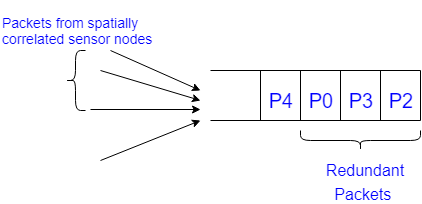
\includegraphics[scale=0.5]{Thesis/figs/5.png}
    \caption{Queue structure at an intermediate node}
    \label{fig:my_label}
\end{figure}
As shown in Figure 2.4, the queuing of redundant packets P2, P3 and P0 will increase the waiting time for non-redundant packet P4.
\end{itemize}
\section{Concluding remarks}
In this chapter, we have presented in depth the work done in existing literature. Taking into consideration the above point mentioned in the research gap, problem formulation and objectives of the proposed work have been discussed in this chapter. 
As can be seen in the chapter, a myriad of endeavour have been made and many issues have been successfully resolved. Utilizing the active queue management for congestion control has to consider several limitations such as limited energy resource and factors such as whether the application in focus is time based or query based. 
The forthcoming chapter will be discussing the proposed scheme to solve the issues discovered in this chapter.
